\chapter{Architektura projektu i użyte technologie}
Podjęty projekt cechuje się wysokim stopniem złożoności oraz potrzebą ciągłej komunikacji i współpracy w zespole. Efektywne zarządzanie infrastrukturą kodu, dokumentacji oraz organizacją prac nakłada obowiązek korzystania z rozwiązań, które umożliwią wspólne planowanie, monitorowanie oraz realizację postępów. W tym rodziale zostaną omówione kluczowe narzędzia użyte w projekcie w ujęciu zarówno narzędzi organizacji pracy - jak i wykorzystanych technologi oraz narzędzi programistycznych.

\section{Narzędzia organizacji pracy}

\textbf{Github} Platforma dostarczająca usługi zdalnego przechowywania oraz kontroli wersji projektów informatycznych. Na potrzeby projektu GitHub został wykorzystany w celu utworzenia repozytorium przechowującego kod źródłowy: aplikacji webowej, aplikacji mobilnej, backendu aplikacji oraz niniejszej pracy wraz ze wszystkimi niezbędnymi assetami i dokumentacją. Repozytorium odgrywa kluczową rolę stanowiąc ważne narzędzie przy organizacji projektu o zadanej złożoności nad którym cały zespół pracuje jednocześnie.

\begin{figure}[H]
    \centering
    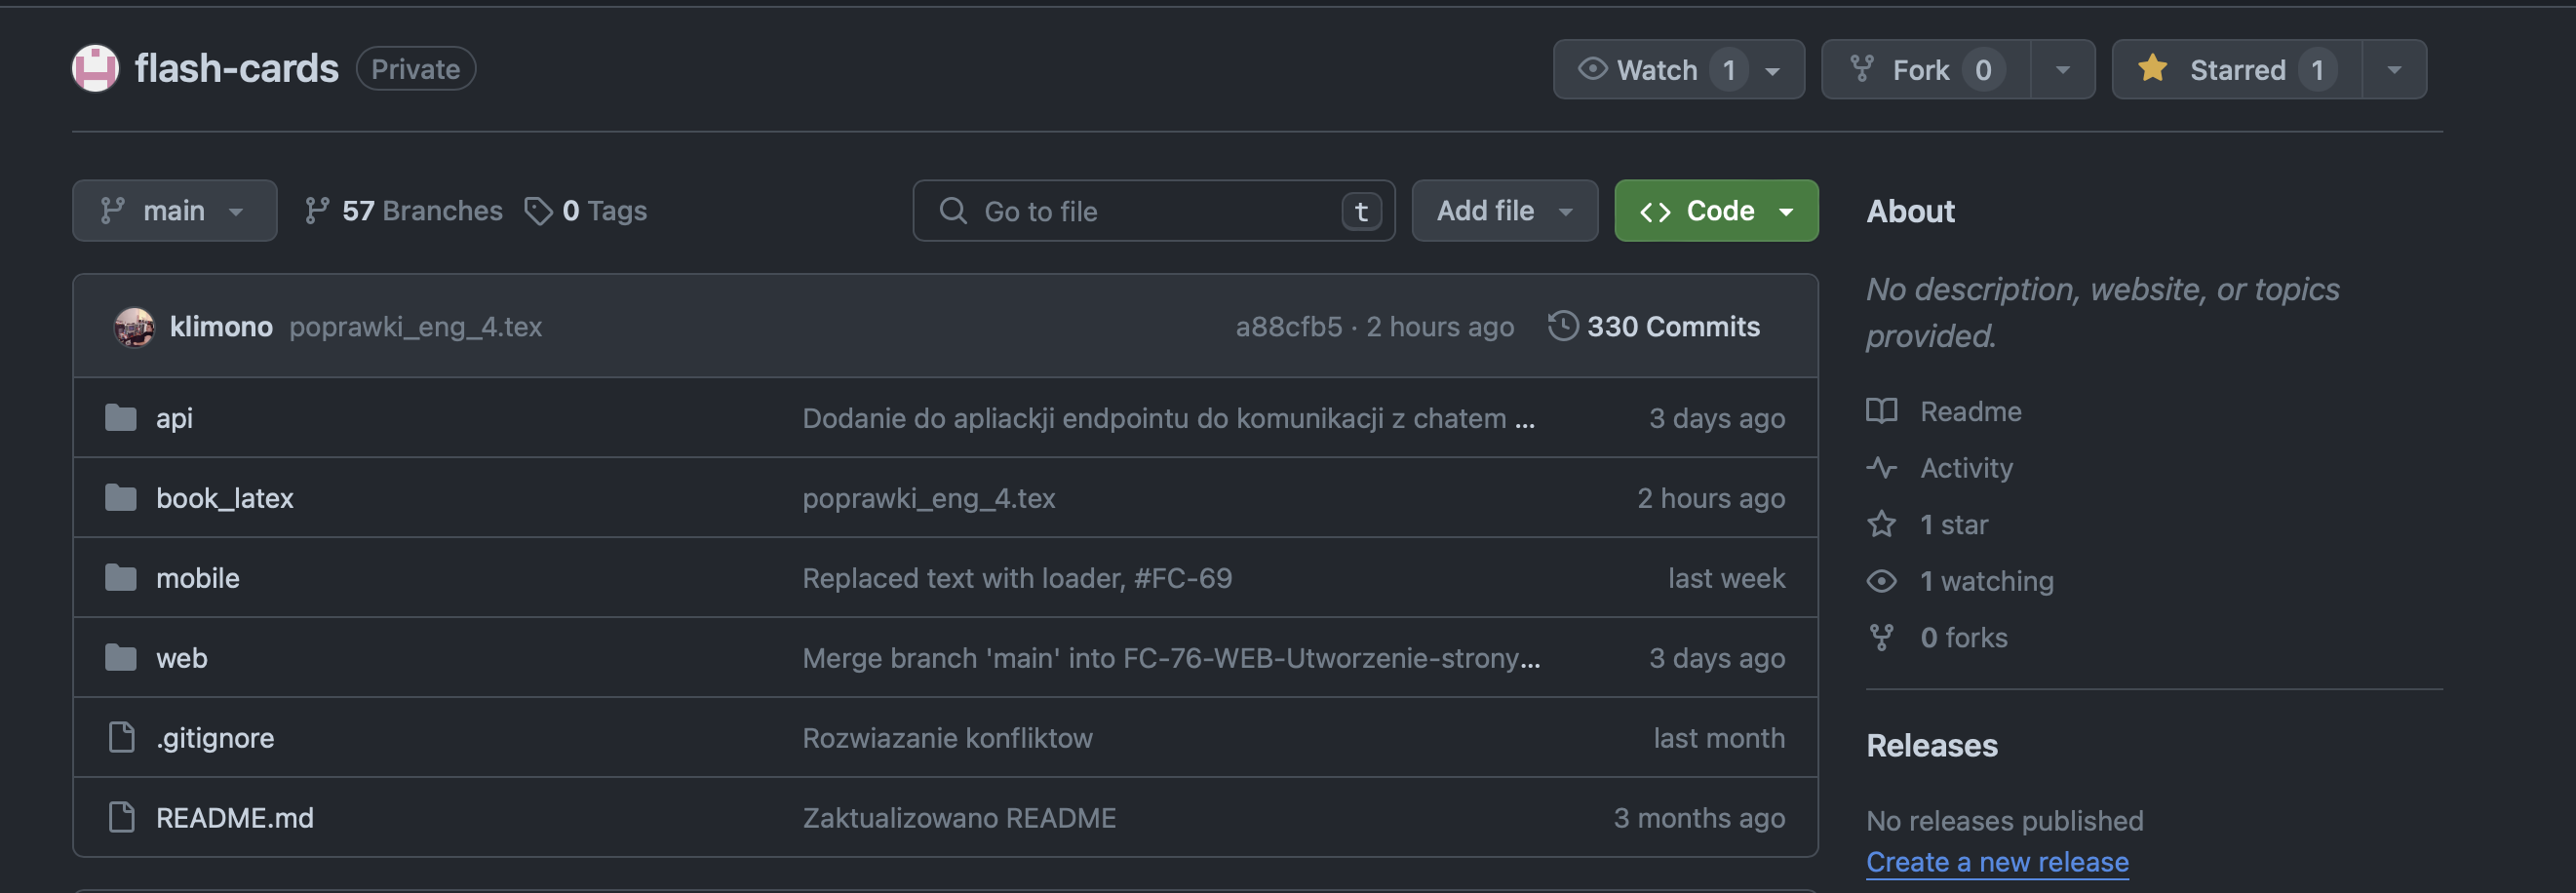
\includegraphics[width=0.9\textwidth]{chapters/chapter_7/github}
    \caption{Repozytorium projektu umieszone na GitHub.}
    \label{img:github}
\end{figure}


\textbf{Jira} Platforma służąca głównie do zarządzania projektami oraz do śledzenia powiązanych z nimi błędów. Jira została wykorzystana w celu dokumentacji, organizacji oraz planowania rozwoju systemu Fishki. Najważniejszą użytą w projekcie funkcją jest możliwość zarządzania sprintami i taskami, takimi jak zadania, bez których realizacja pracy w wybranym modelu byłaby niemożliwa.

\begin{figure}[H]
    \centering
    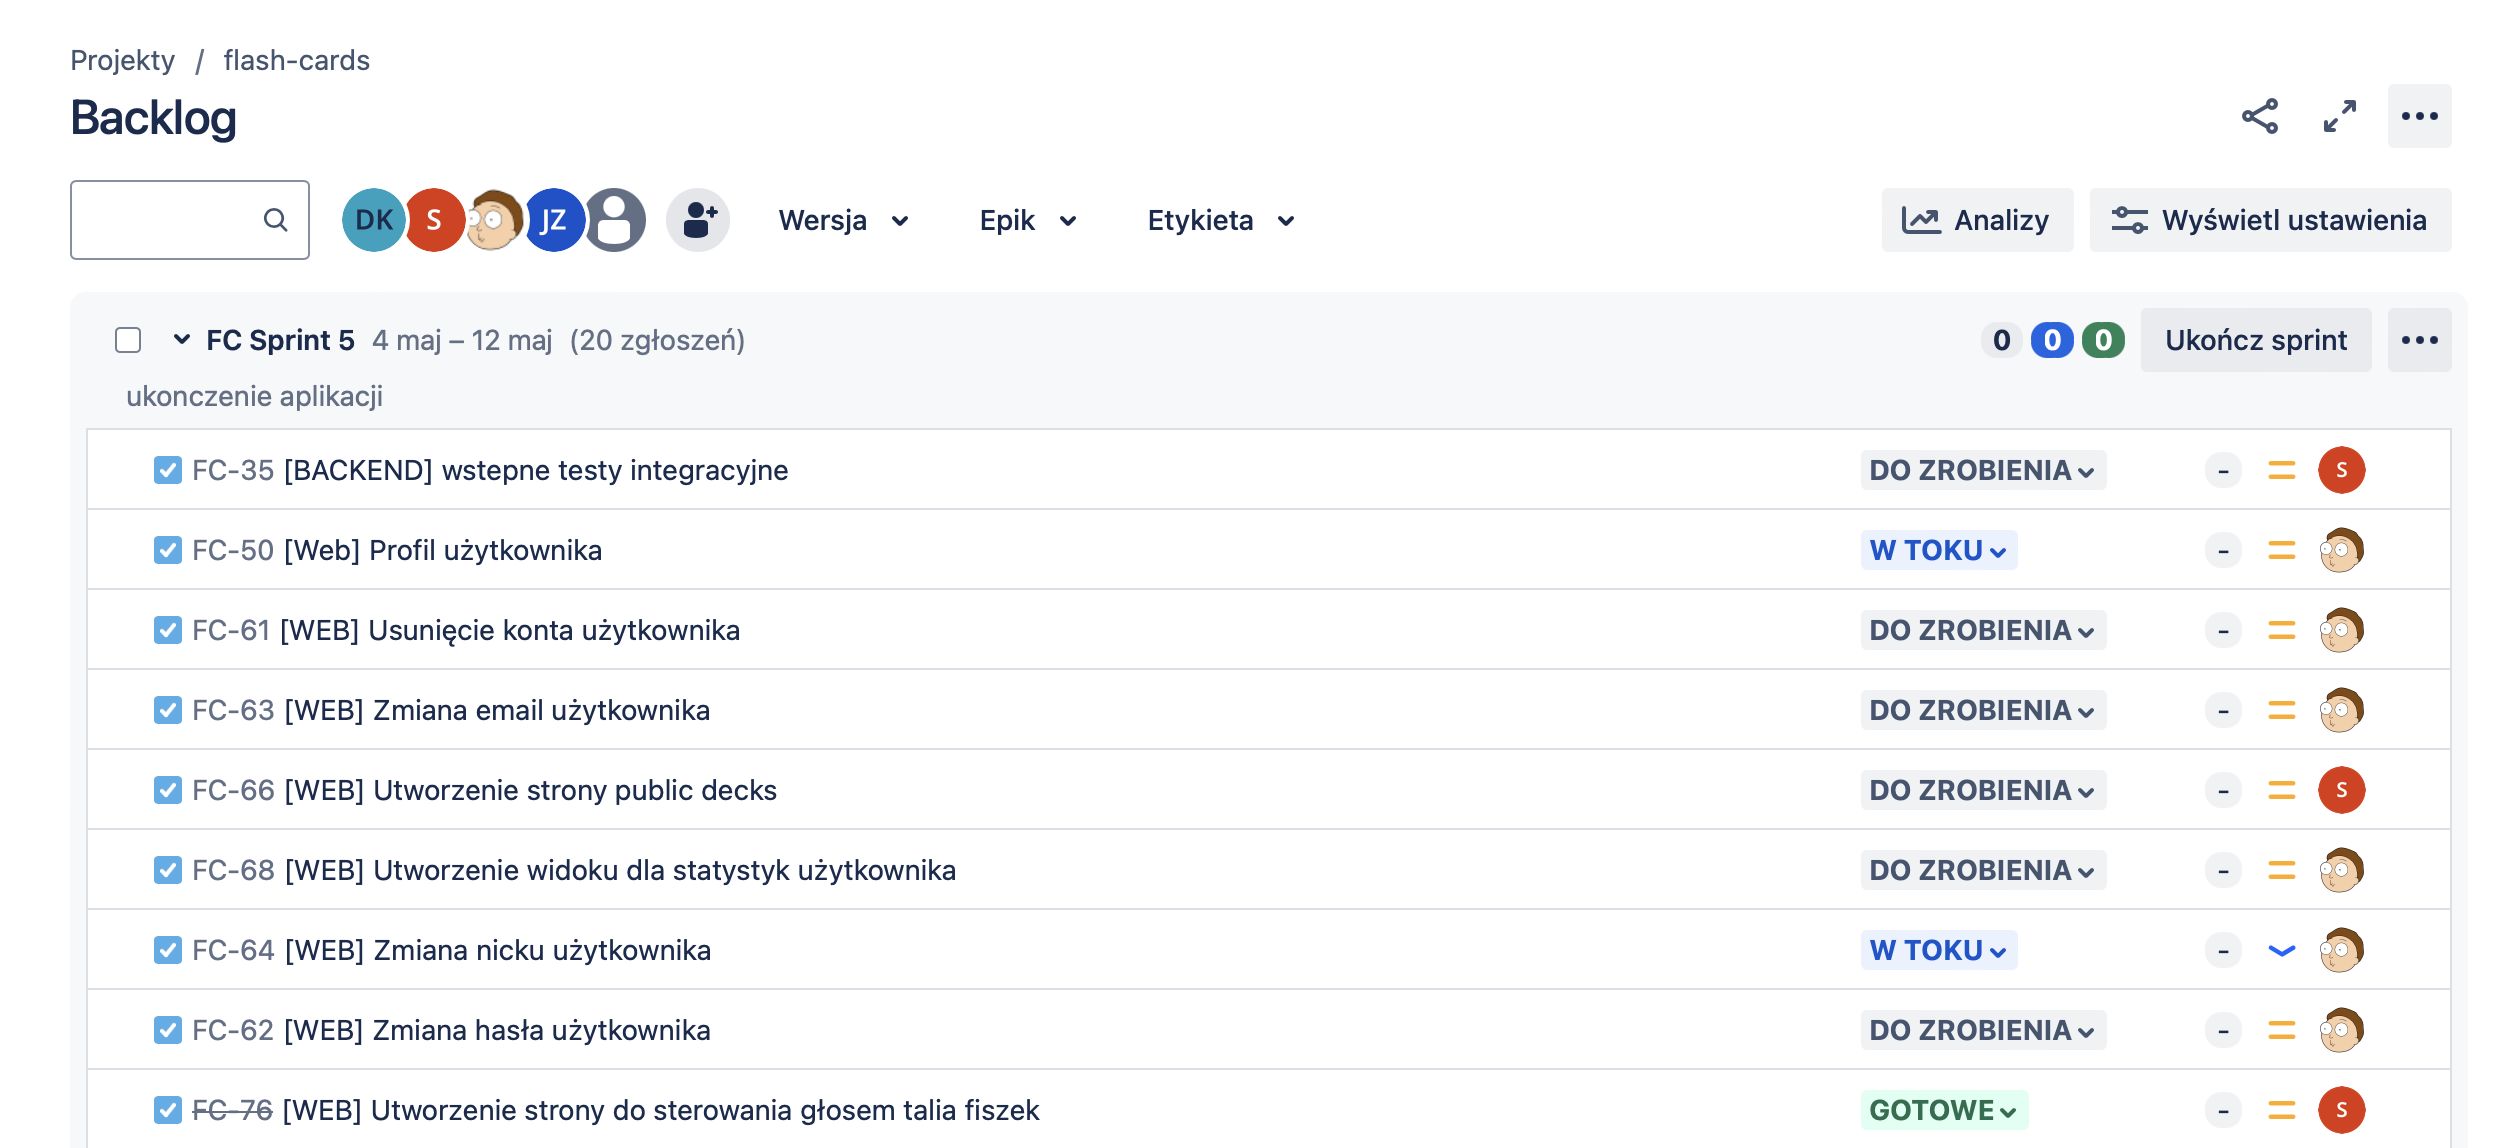
\includegraphics[width=0.9\textwidth]{chapters/chapter_7/jira}
    \caption{Sprint rozpisany przy pomocy Jira.}
    \label{img:jira}
\end{figure}


\textbf{Miro} Wirtualna tablica umożliwiająca współpracę zespołową w czasie rzeczywistym. Miro zostało użyte do połączenia ze sobą mockupów aplikacji mobilnej utworzonych w canvie.

\begin{figure}[H]
    \centering
    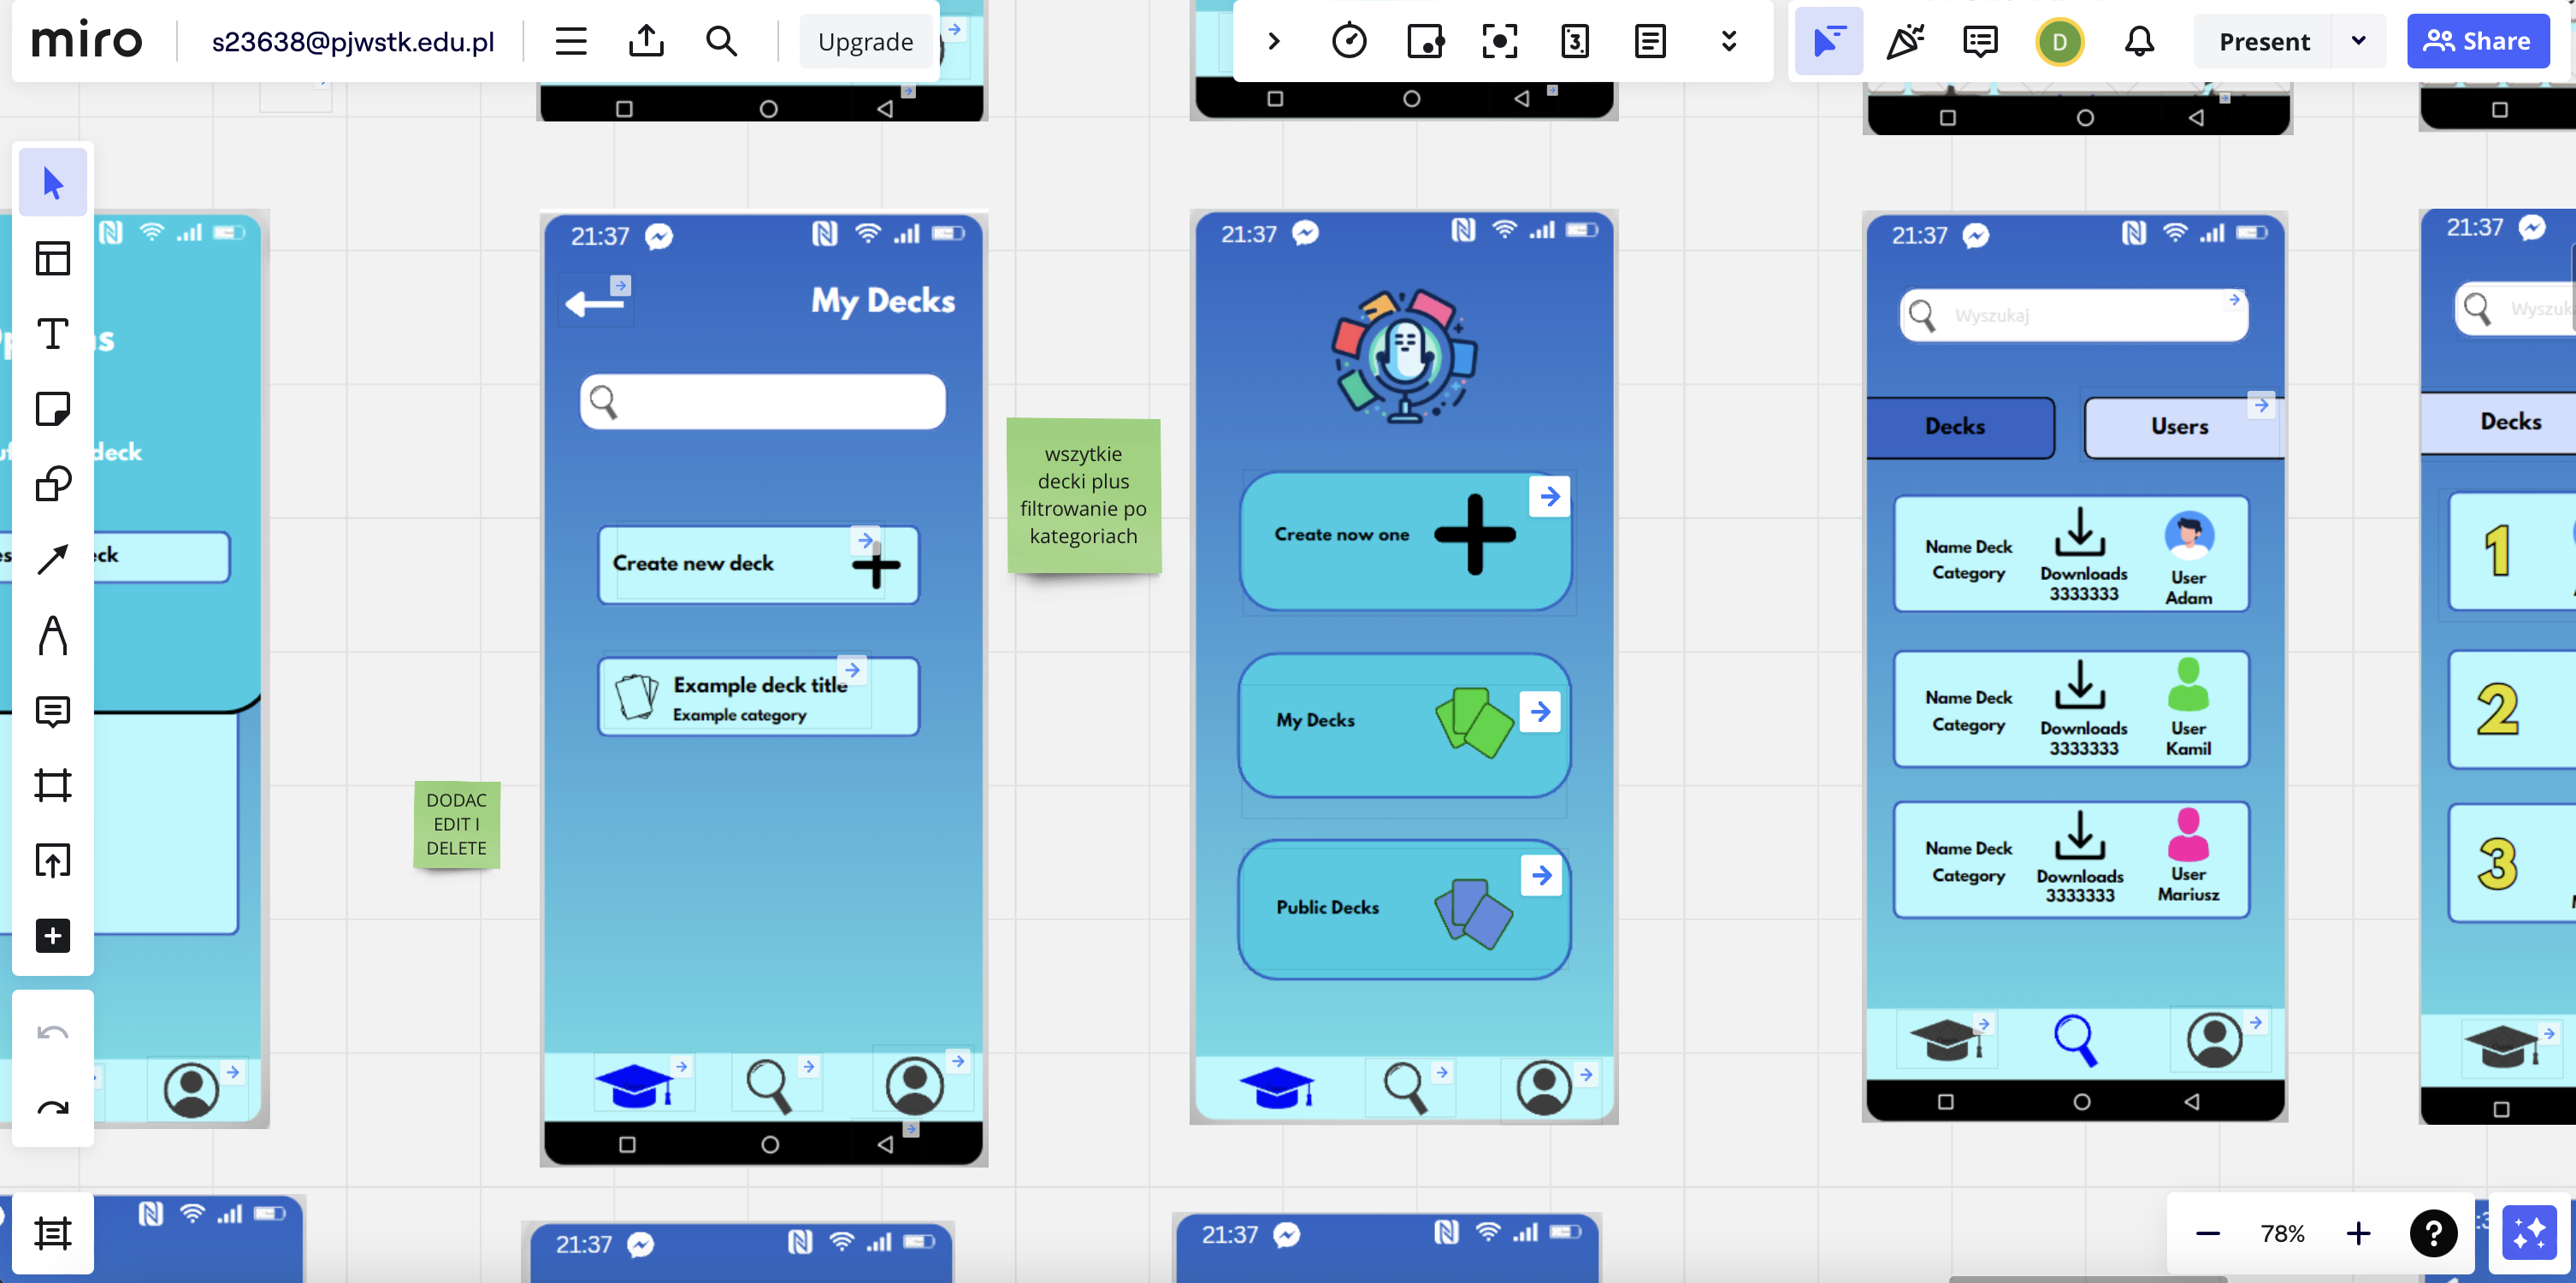
\includegraphics[width=0.9\textwidth]{chapters/chapter_7/miro}
    \caption{Tablica w Miro z interaktywnymi mockupami projektu.}
    \label{img:miro}
\end{figure}


\textbf{Google Drive} Usługa pozwalająca na przechowywanie plików wirtualnie w chmurze. Wykorzystana w projekcie do zarządzania i przechowywania niektórych dokumentów związanych z projektem.

\begin{figure}[H]
    \centering
    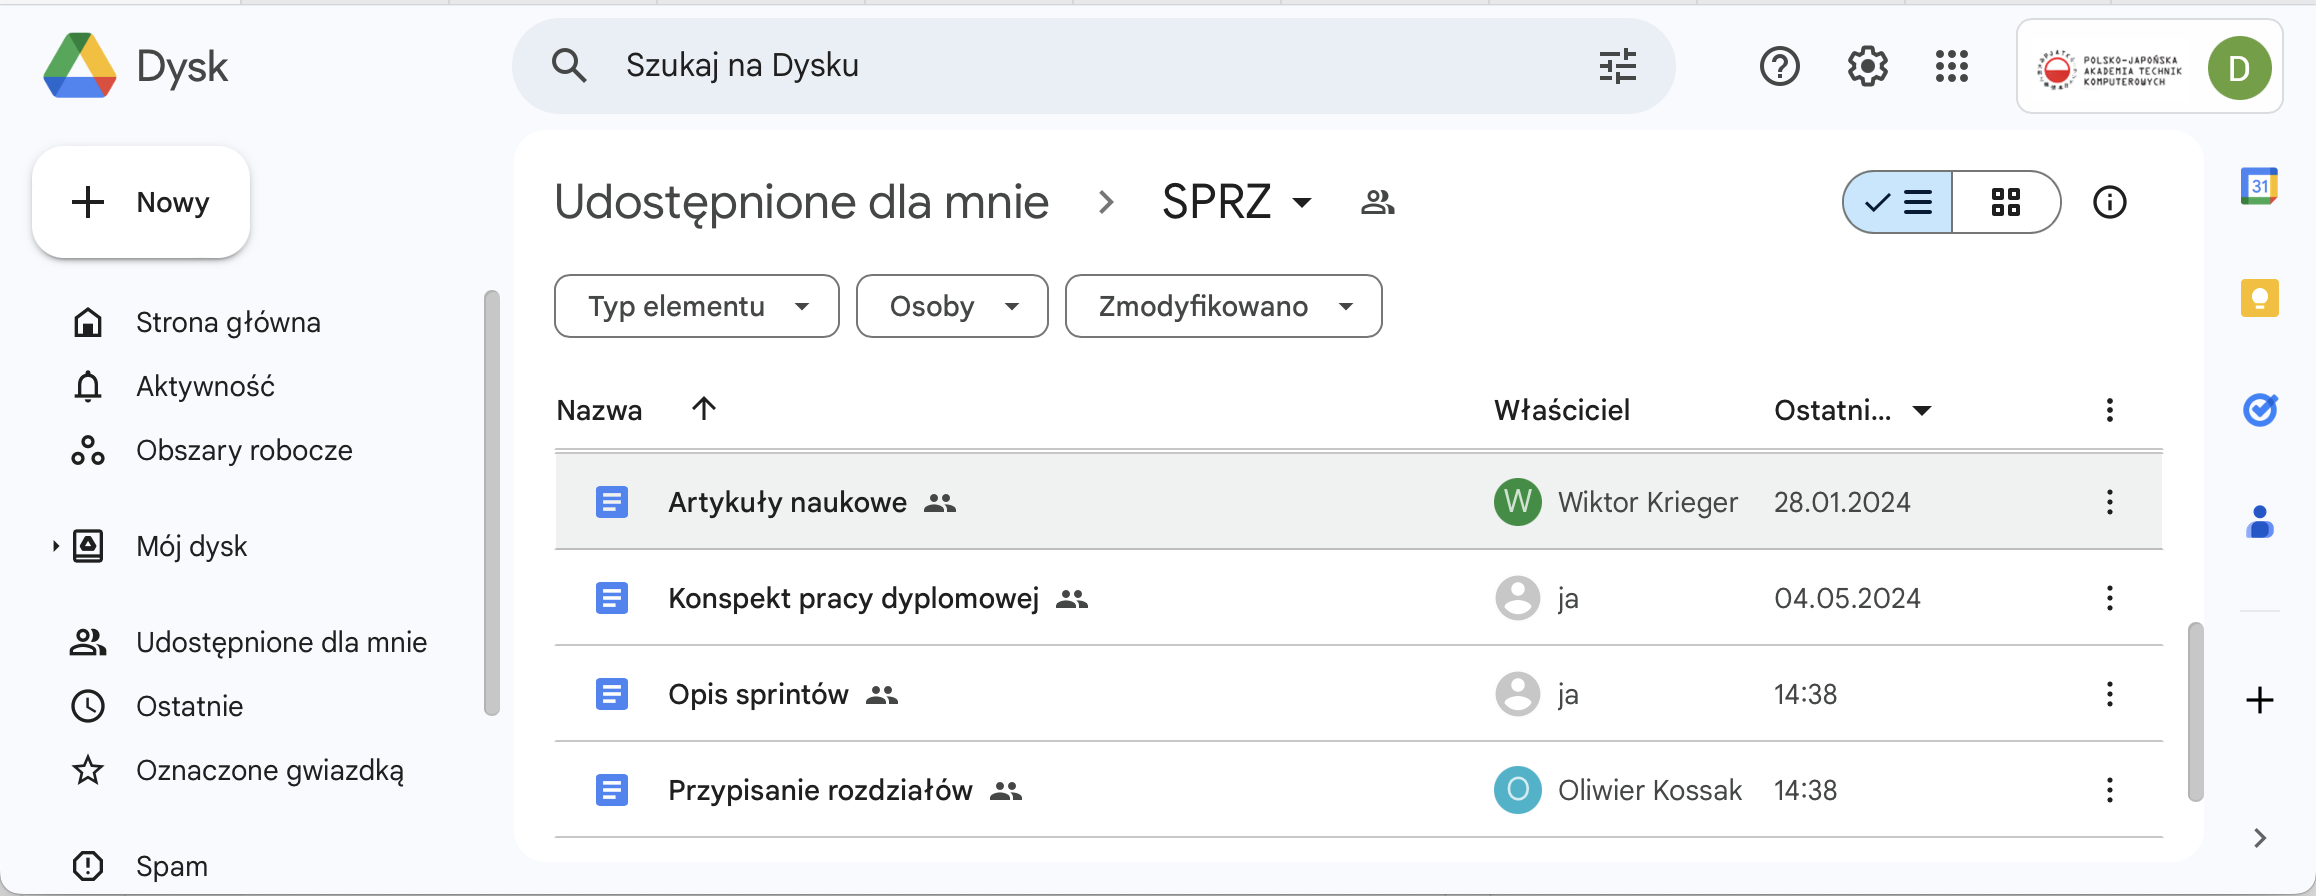
\includegraphics[width=0.9\textwidth]{chapters/chapter_7/google_drive}
    \caption{Dokumenty przechowywane na Google Drive.}
    \label{img:google_drive}
\end{figure}


\textbf{Canva} Bezpłatne narzędzie służące do tworzenia grafik i stron internetowych. Program został użytu w celu utworzenia mockapów aplikacji moblinej oraz diagramu architektury.

\begin{figure}[H]
    \centering
    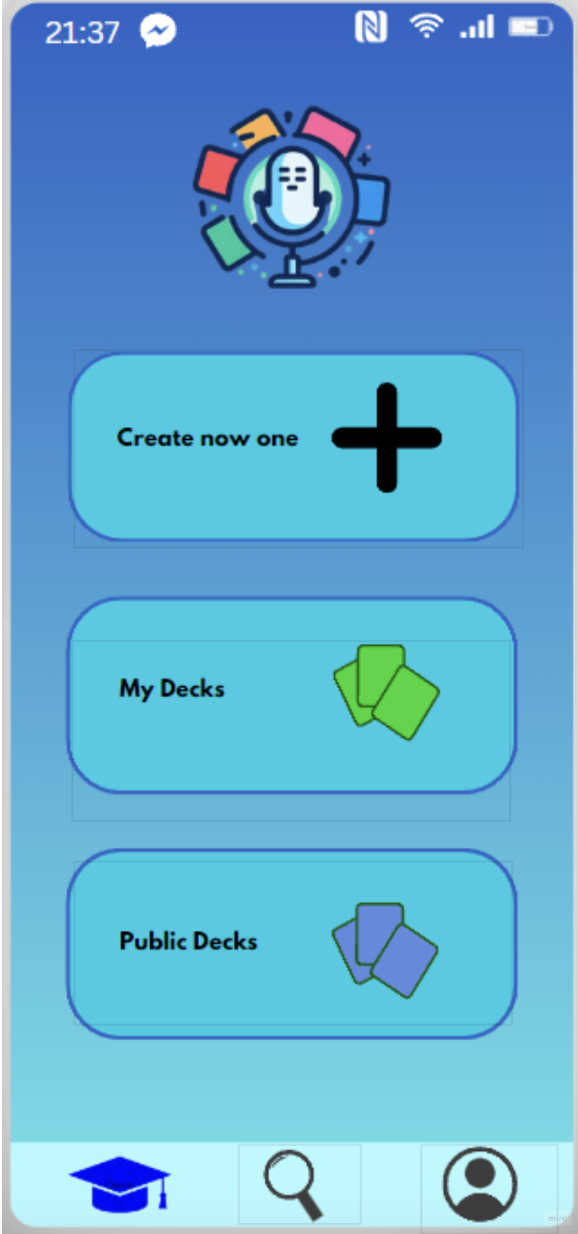
\includegraphics[width=0.3\textwidth]{chapters/chapter_7/canva}
    \caption{Grafika mockupu wykonana w Canva.}
    \label{img:canva}
\end{figure}


\textbf{Discord} Bezpłatny program służący do komunikacji głosowej i tekstowej. Wykorzystywany do spotkań organizacyjnych i komunikacji członków zespołu o problemach związanych z projektem.

\medskip

\textbf{Enterprise Architect} Program służący do modelowania diagramów. Został wykorzystany do przygotowania diagramu przypadków użycia.

\medskip

\textbf{dbdiagram.io} Narzędzie online wykorzystywane przy projektowaniu diagramów.. W projekcie zostało użyte do stworzenia diagramu ERD.

\medskip

\textbf{LaTeX} System składu tekstu. Wykorzystany w projekcie do organizacji oraz tworzenia książki projektu.

\medskip

\textbf{Git} Rozproszony system kontroli wersji, wykorzystany w projekcie do zarządzania kodem.

\section{Aplikacja webowa}

\textbf{React} Biblioteka JavaScript wykorzystywana do tworzenia interfejsów użytkownika, pozwala ona na szybkie i łatwe kreowanie uniwersalnych komponentów, umożliwia to wykorzystanie jednego komponentu w wielu miejscach w kodzie. Biblioteka została wykorzystana do tworzenia strony internetowej.

\medskip

\textbf{Typescript} Rozszerza JavaScript o możliwość typowania zmiennych. TypeScript został wykorzystany w celu szybszego wykrywania błędów w kodzie i łatwiejszym zarządzaniu go.

\medskip

\textbf{Material UI} Popularna biblioteka UI, zawiera zestaw komponentów do tworzenia interfejsów internetowych. Używana w połączeniu z biblioteką React.js.

\medskip

\textbf{Node JS} Środowisko, które pozwala na uruchomienie javascriptu na serwerze jako samodzielną aplikację.

\section{Aplikacja mobilna}

\textbf{React Native} Framework pozwalający na tworzenie natywnych aplikacji mobilnych dla iOS i Android przy użyciu JavaScript i Reacta. Umożliwia programistom wykorzystanie jednego kodu źródłowego do budowy aplikacji na obie wymienione platformy.

\medskip

\textbf{Expo} Framework i platforma służąca do tworzenia aplikacji na iOS i Android za pomocą React Native, która ułatwia rozwój aplikacji mobilnych

\medskip

\textbf{Typescript} Jw. w sekcji “Aplikacja webowa”.

\section{Backend aplikacji}

\textbf{Python} Wysokopoziomowy język programowania. Wykorzystany w projekcie ze względu na swoją prostotę, wszechstronność i wieloplatformowość.

\medskip

\textbf{FastAPI} Framework do tworzenia interfejsów API w języku Python. Wykorzystany w projekcie ze względu na szybkość co pozwala na szybką komunikację z bazą danych. Framework wykorzystuje asynchroniczną obsługę żądań co pozwala aplikacji osiągnąć wysoką wydajność.

\section{Baza danych}

\textbf{MariaDB} Relacyjna baza danych, wykorzystana w projekcie ze względu na
wysoką wydajność, a także otwartoźródłowy charakter systemu.

\section{Infrastruktura serwerowa}

\textbf{Microsoft Azure} Platforma chmurowa pozwalająca wdrożyć wirtualną infrastrukturę IT. Wykorzystana na rzecz utrzymania środowiska projektowego tj. kontenera z Api, backend aplikacji webowej i bazę danych w oparciu o wirtualną maszynę z systemem operacyjnym Ubuntu server.

\textbf{Serwer Nginx} Zaawansowany serwer WWW i serwer PROXY. Wykorzystany w celu pełnej konfiguracji aplikacji webowej, HTTPS i przekierowania ruchu ze strony do API.

\section{Narzędzia programistyczne}

\textbf{Jetbrains PyCharm} Środowisko programistyczne zaprojektowane dla języka Python. Wykorzystane w projekcie podczas projektowania i tworzenia backendu aplikacji oraz do kompilacji książki w LaTeX.

\medskip

\textbf{Jetbrains WebStorm} Środowisko programistyczne zaprojektowane głównie dla języka JavaScript oraz technologii wykorzystywanych w budowie aplikacji webowej/mobilnej. Użyte w projektowaniu oraz tworzeniu frontendu.

\medskip

\textbf{Docker} Narzędzie programistyczne, które umożliwia tworzenie, wdrażanie i uruchamianie aplikacji w kontenerach. Docker wykorzystany został do umieszczenia aplikacji webowej, api i bazy danych w kontenerach, aby ułatwić łatwe uruchamiania aplikacji.

\medskip

\textbf{Visual Studio Code} Środowisko programistyczne wszechstronnego przeznaczenia. Wykorzystane na etapie tworzenia aplikacji ze względu na dodatek Thunder Client, który zastąpił popularnego Postmana, do testowania api.

\medskip

\textbf{Android Studio} Oficjalne zintegrowane środowisko programistyczne dla systemu operacyjnego Google Android. Umożliwia ściąganie różnych wersji emulatorów, ściągania wymaganych paczek do uruchomienia danego emulatora, a także do celów testowania wytwarzanej aplikacji mobilnej.

\medskip

\textbf{Xcode} Oficjalne środowisko programistyczne Apple udostępniające narzędzia do tworzenia aplikacji oraz oprogramowania dla systemów z rodziny iOS i macOS. Wykorzystane w projekcie w celu testowania aplikacji mobilnej w symulatorach urządzeń z zainstalowanym systemem iOS.

\medskip

\textbf{Adobe Illustrator} Rozbudowany program graficzny przeznaczony do tworzenia i edycji grafiki wektorowej. Utworzone zostały za jego pomocą ikony oraz tło do naszych aplikacji.
